%\begin{frame}
%\frametitle{Euler-Lagrange Equations}
%At the solution, the derivatives of the objective function are zero, which means that the velocity at any time point is given by:
%\begin{eqnarray*}
%{\bf L}^{\dagger}{\bf L}{\bf v}_{t} = \frac{1}{\sigma^2} \det |{\bf D}( {\boldsymbol\varphi}_{1} \circ {\boldsymbol\varphi}_{t}^{-1}) | (\nabla (\mu \circ {\boldsymbol\varphi}_{t}^{-1})) (\mu \circ {\boldsymbol\varphi}_{t}^{-1} - f \circ {\boldsymbol\varphi}_1 \circ {\boldsymbol\varphi}_{t}^{-1}) 
%\end{eqnarray*}

%If we introduce something that we'll call initial momentum:
%\begin{eqnarray*}
%{\bf u}_{0} = {\bf L}^{\dagger}{\bf L} {\bf v}_0 = \frac{1}{\sigma^2} \det | {\bf D}{\boldsymbol\varphi}_{1} | (\nabla \mu) (\mu - f \circ {\boldsymbol\varphi}_1)
%\end{eqnarray*}
%we see that the velocity at any time point is determined by the initial momentum (or velocity), according to:
%\begin{eqnarray*}
%{\bf v}_{t} = \left({\bf L}^{\dagger}{\bf L}\right)^{-1} \left(\det |{\bf D}{\boldsymbol\varphi}_{t}^{-1}| ({\bf D}{\boldsymbol\varphi}_{t}^{-1})^T ({\bf u}_{0} \circ {\boldsymbol\varphi}_{t}^{-1}) \right)
%\end{eqnarray*}
%\end{frame}

\begin{frame}
\frametitle{Geodesic Shooting}
At the solution, gradients of the objective function should vanish:
\begin{align*}
{\bf L}^{\dagger}{\bf L} {\bf v}_{0} + \frac{1}{\sigma^2} \det | {\bf D}{\boldsymbol\varphi}_{1} | (f \circ {\boldsymbol\varphi}_1 - \mu)(\nabla \mu) = 0
\end{align*}

Re-expressiong this, we see that the initial velocity and momentum is given by:
\begin{align*}
{\bf L}^{\dagger}{\bf L} {\bf v}_{0} = {\bf u}_0 = {\frac{1}{\sigma^2} (\nabla \mu)} {\det | {\bf D}{\boldsymbol\varphi}_{1} | (\mu - f \circ {\boldsymbol\varphi}_1)}
\end{align*}
\end{frame}

%%%%%%%%%%%%%%%%%%%%%%%%%%%%%%%%%%%%%%%%%%%%%%%%%%%%%%%%%%%%%%%
\begin{frame}
\frametitle{``Scalar Momentum''}
\begin{eqnarray*}
{\bf u}_{0} = \color{blue}{\frac{1}{\sigma^2} (\nabla \mu)} \color{red}{\det | {\bf D}{\boldsymbol\varphi}_{1} | (\mu - f \circ {\boldsymbol\varphi}_1)}
\end{eqnarray*}
If a population of subjects are all aligned with the same template image, $\color{blue}{\frac{1}{\sigma^2} (\nabla \mu)}$ will be the same for all subjects.
Deviations from the template are encoded by the ``\emph{scalar momentum}'', $\color{red}{\det | {\bf D}{\boldsymbol\varphi}_{1} |(\mu - f \circ {\boldsymbol\varphi}_1)}$.
This is a scalar field, and in principle is all that is needed (along with the template) to reconstruct the original images.\par
\vspace{.25cm}
\begin{tiny}
Miller et al. ``Collaborative computational anatomy: an MRI morphometry study of the human brain via diffeomorphic metric mapping.'' Human Brain Mapping 30(7):2132--2141 (2009).\par
Singh, Fletcher, Preston, Ha, King, Marron, Wiener \& Joshi (2010). \emph{Multivariate Statistical Analysis of Deformation Momenta Relating Anatomical Shape to Neuropsychological Measures}. T. Jiang et al. (Eds.): MICCAI 2010, Part III, LNCS 6363, pp. 529--537, 2010.\par
\end{tiny}
\end{frame}

\begin{frame}
\frametitle{Evolution}
\begin{center}
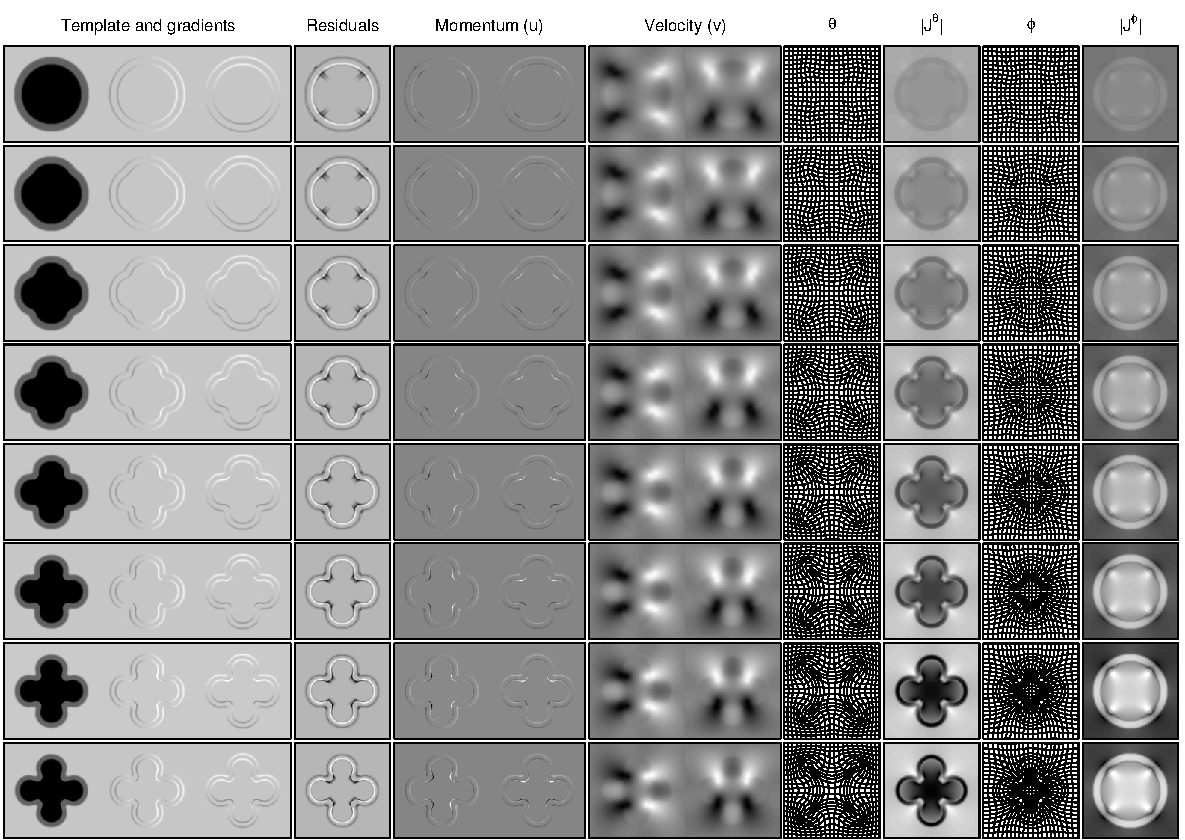
\includegraphics[width=.9\textwidth]{evolution}
\end{center}
\end{frame}


%%%%%%%%%%%%%%%%%%%%%%%%%%%%%%%%%%%%%%%%%%%%%%%%%%%%%%%%%%%%%%%

\begin{frame}
\frametitle{Example Images}
Some example images.
\begin{center}
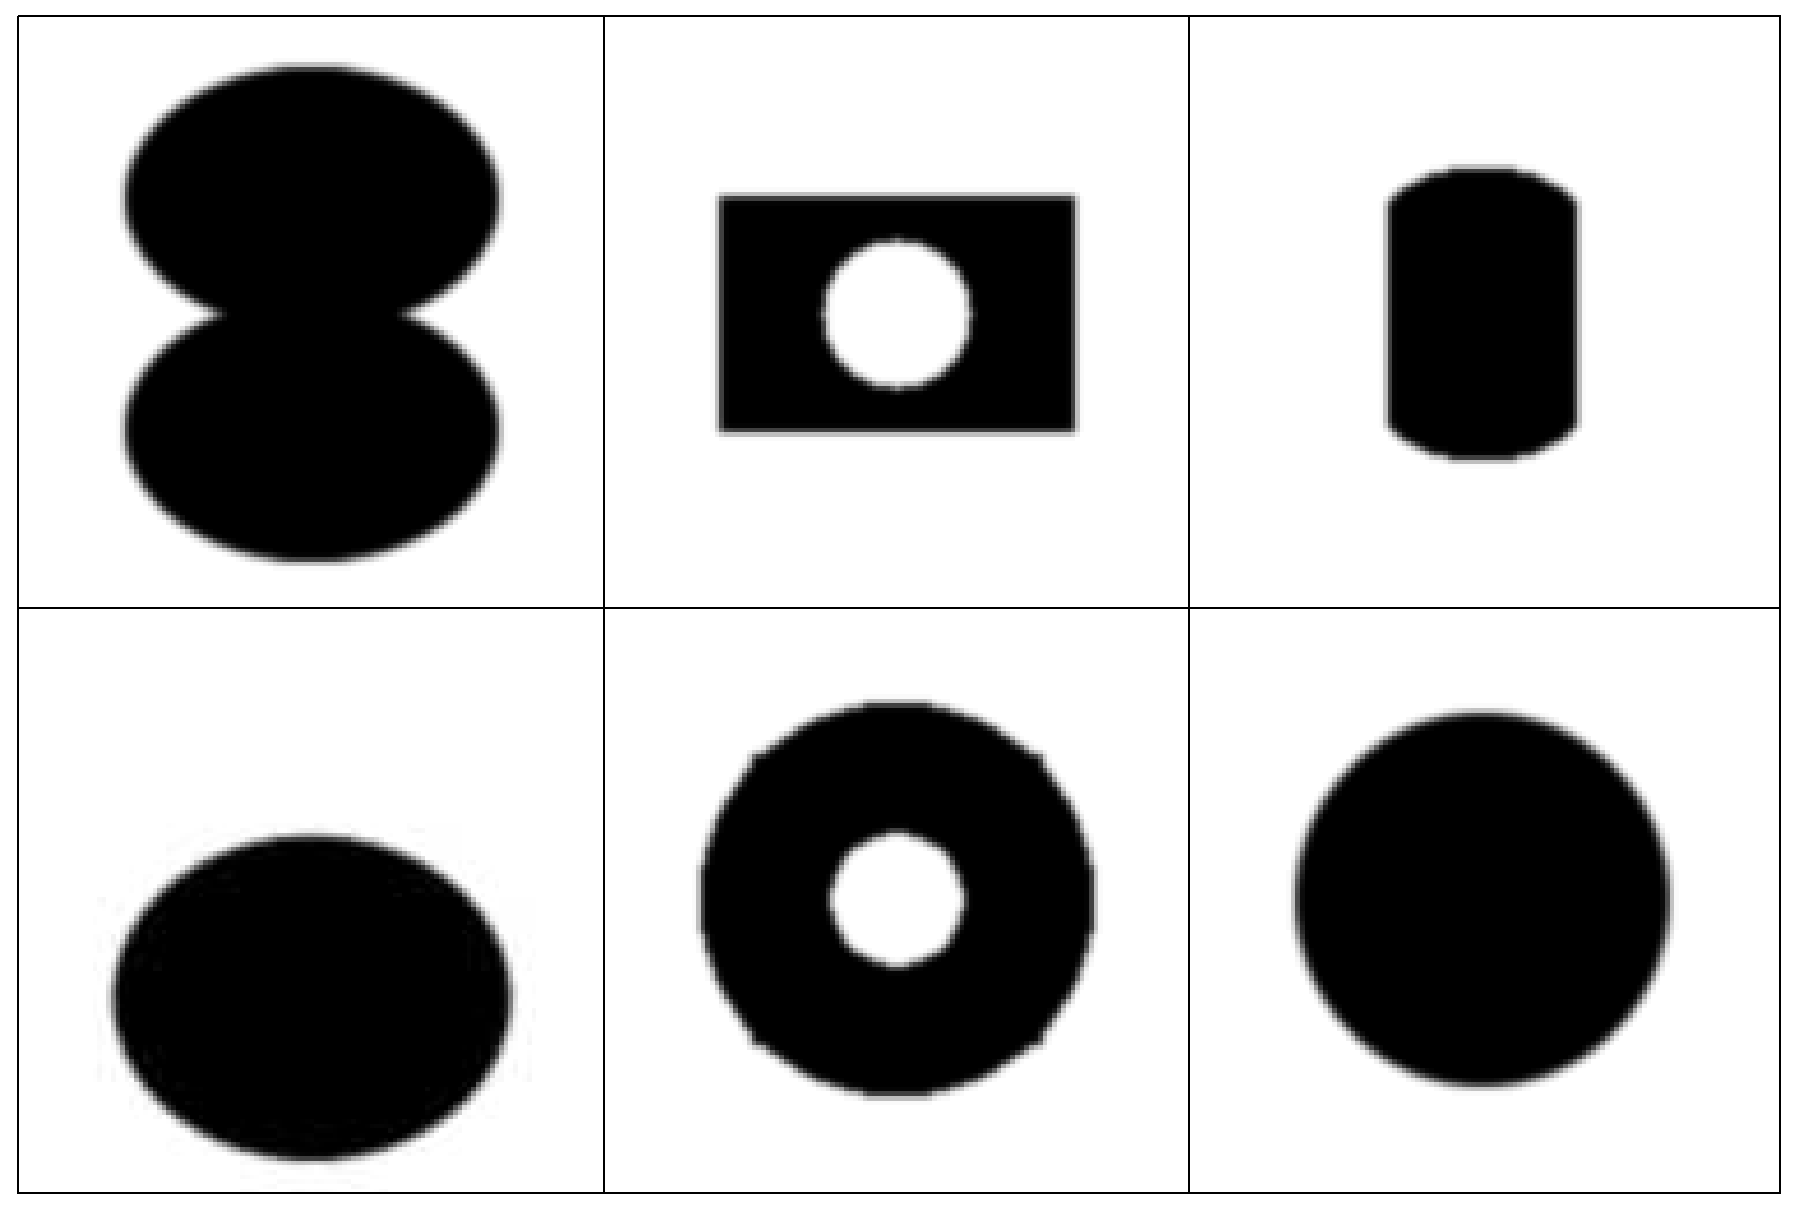
\includegraphics[width=0.9\textwidth]{original}
\end{center}
\end{frame}

%%%%%%%%%%%%%%%%%%%%%%%%%%%%%%%%%%%%%%%%%%%%%%%%%%%%%%%%%%%%%%%

\begin{frame}
\frametitle{Scalar Momentum}
Scalar momentum after aligning the examples to a common template.
\begin{center}
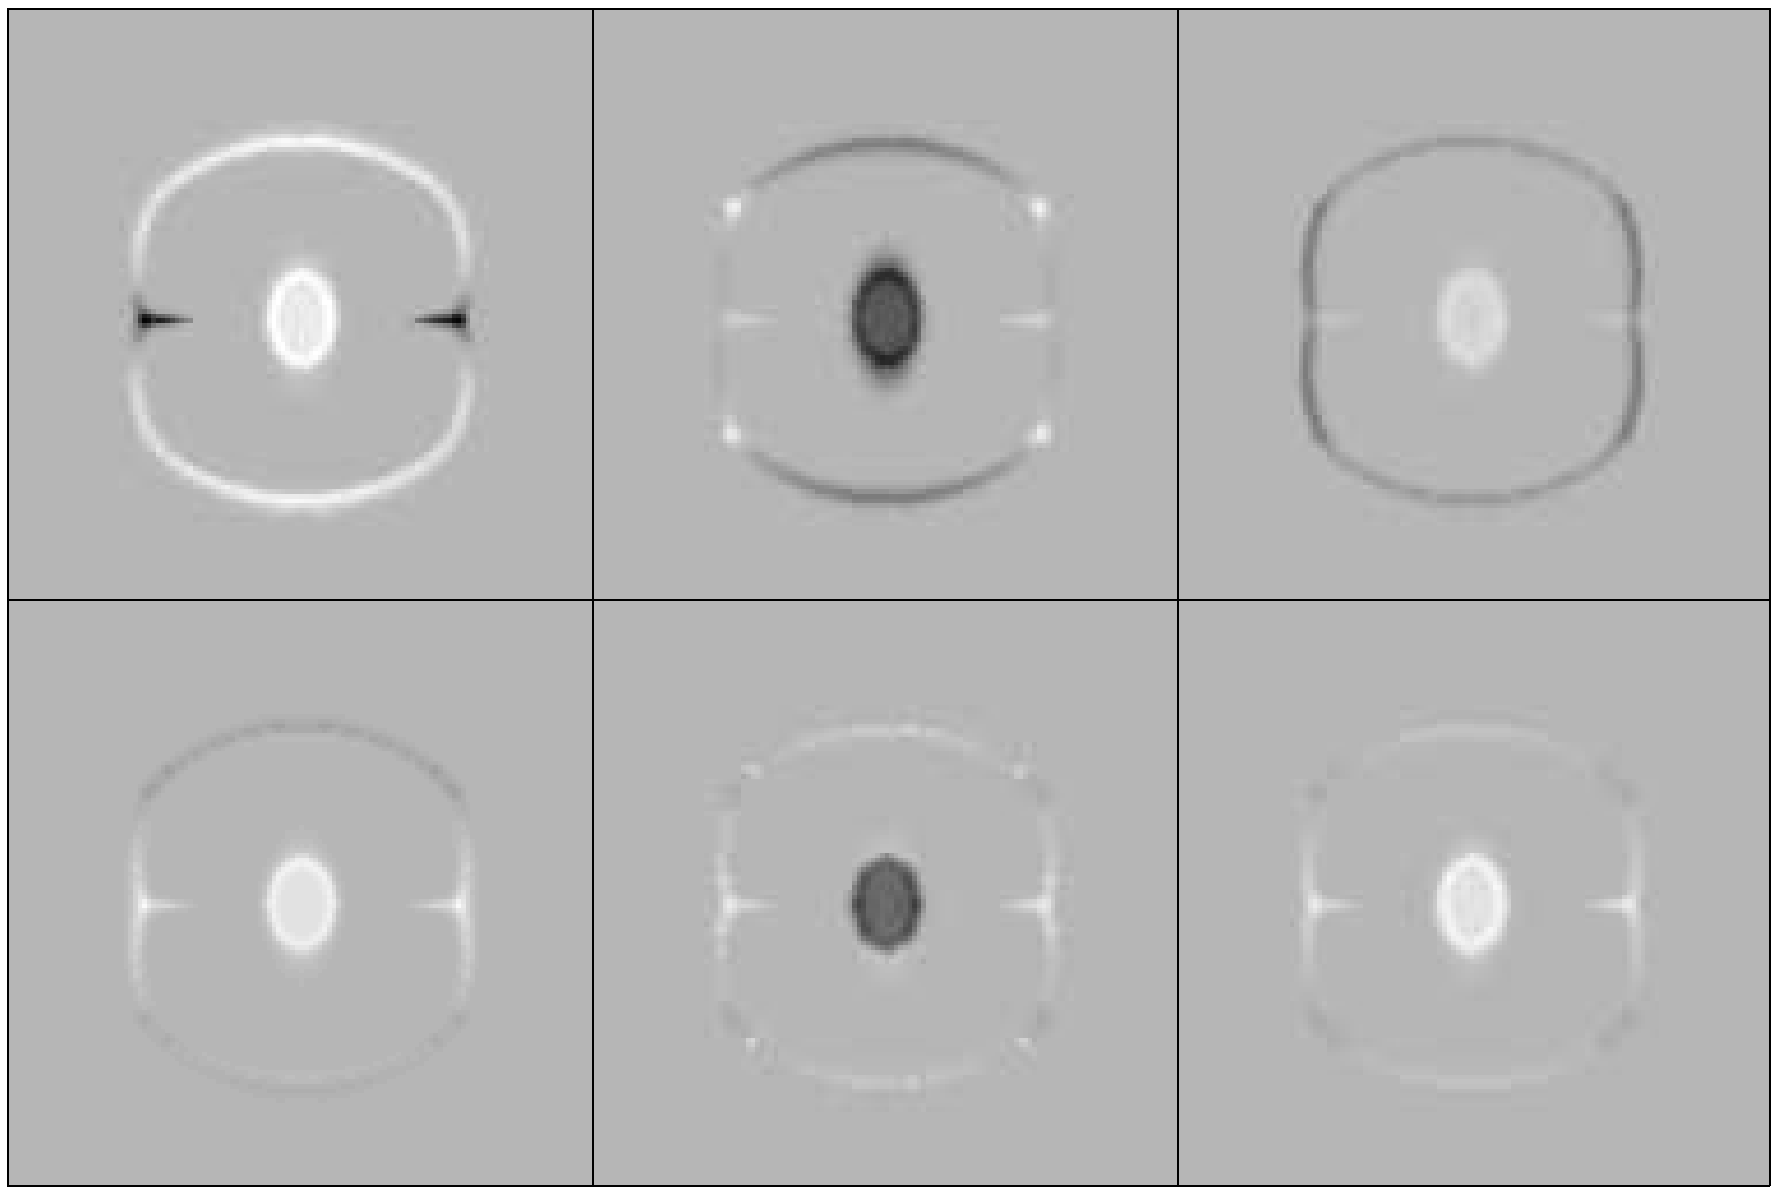
\includegraphics[width=0.9\textwidth]{alpha}
\end{center}
\end{frame}

%%%%%%%%%%%%%%%%%%%%%%%%%%%%%%%%%%%%%%%%%%%%%%%%%%%%%%%%%%%%%%%

\begin{frame}
\frametitle{Reconstructed Images}
Images reconstructed using just the template and scalar momentum.
\begin{center}
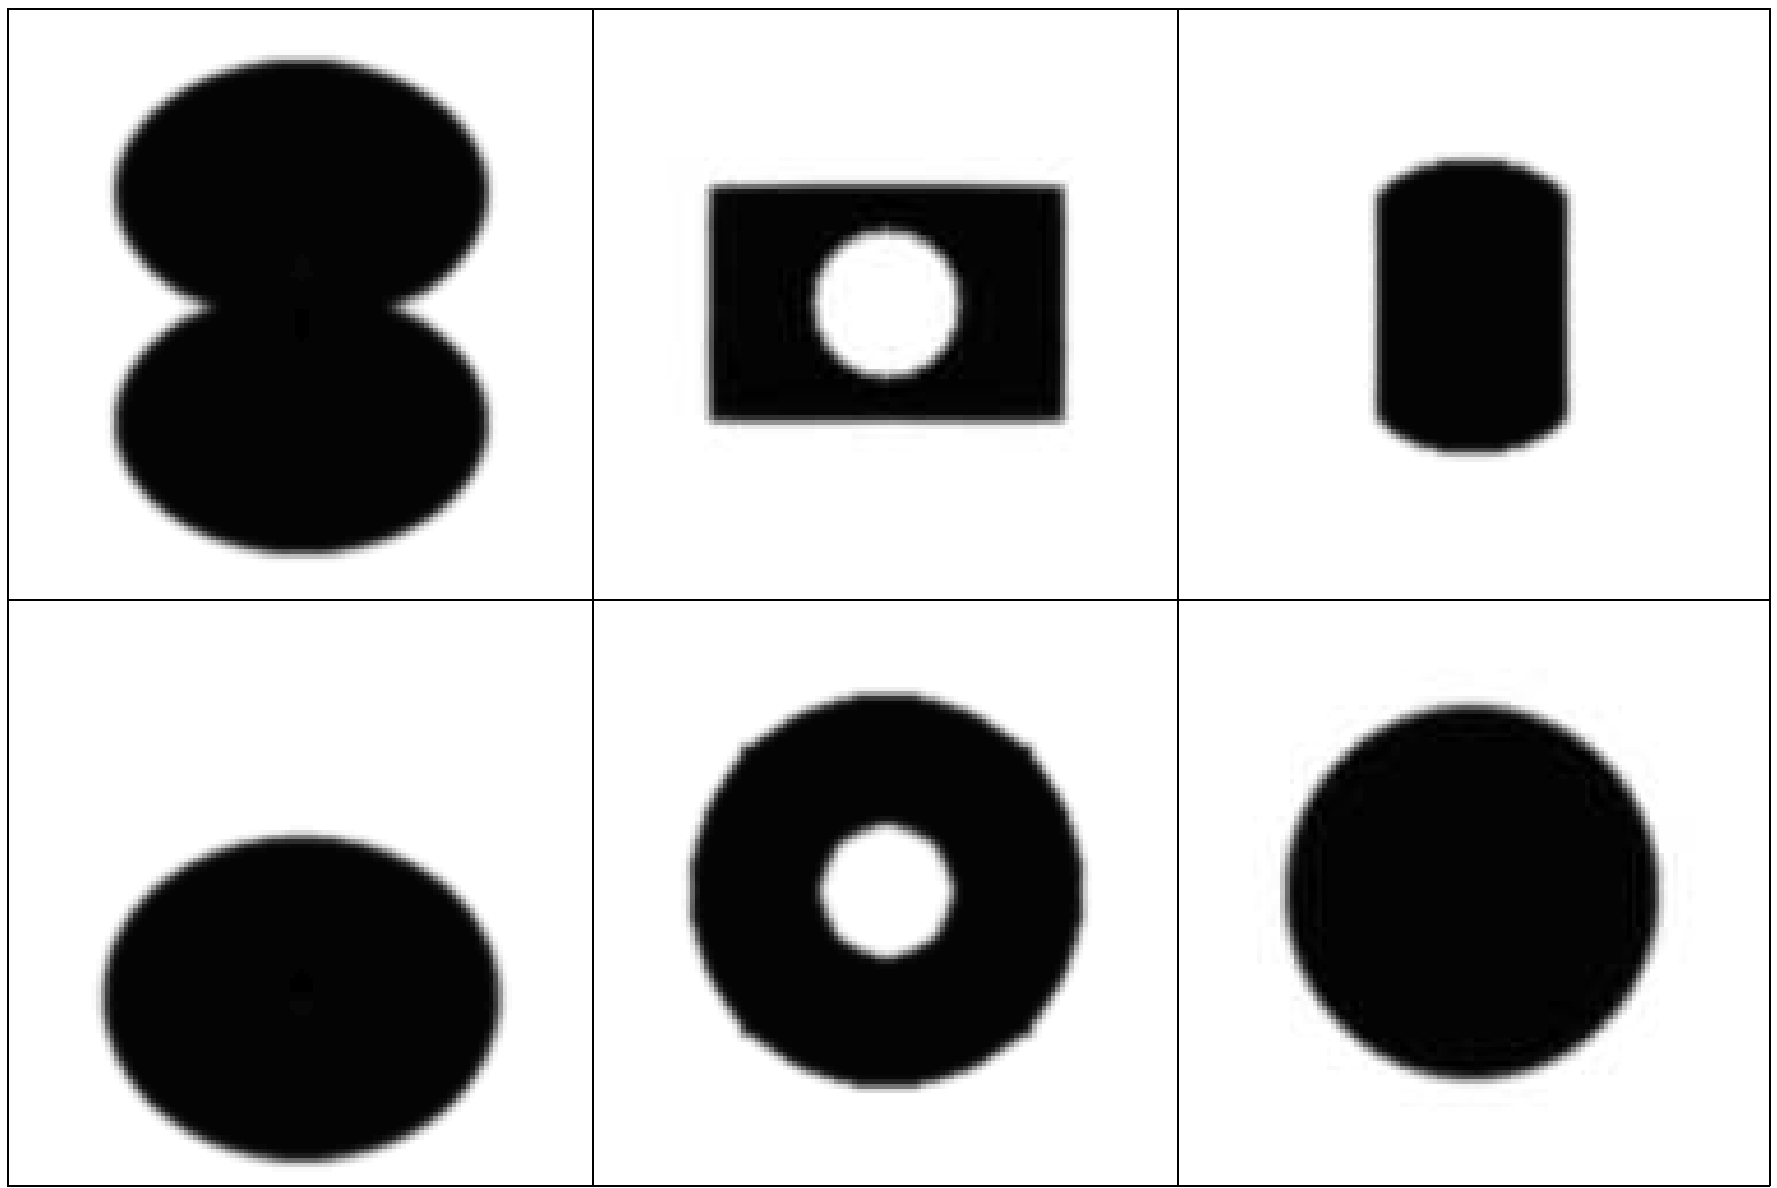
\includegraphics[width=0.9\textwidth]{reconstructed}
\end{center}
\end{frame}

%%%%%%%%%%%%%%%%%%%%%%%%%%%%%%%%%%%%%%%%%%%%%%%%%%%%%%%%%%%%%%%


